\section{Longest Common Subsequence (LCS) }
Another widely used metrics in the time-series similarity is the Longest Common Subsequence or LCS. LCS could be seen as the successor of the application of the Euclidean distance, DTW or scales and shifts \cite{citeulike:3816327} since it might be essentially based on any of these. 

The idea of LCS is explained in the classical Computer Science manuscript \cite{citeulike:180287} for the string matches and perfectly described in \cite{citeulike:4367061} for the real values and feature sequences. While Yazdani and Ozsoyoglu designed their algorithm specifically for image sequences their explain it as an algorithm of matching real-valued sequences and specifically pointed application to time-series and time-series features as Fourier coefficients etc. The Figure \ref{fig:lcs} taken from the article and explains the approach taken: each of the images is approximated by the set of the specific to the domain real-values, and if $R$ and $S$ match than $FR$ and $FS$ match anlagously, if $FR$ and $FS$ are similar than $R$ and $S$ are similar, but we will extend the (image) decomposition approach in the next chapter, here we will focus on the LCS algorithm.

\begin{figure}[tbp]
   \centering
   \includegraphics[height=40mm]{lcs.eps}
   %%{seriesheatmap}
   \caption{This figure is taken from \cite{citeulike:4367061} and while it designed to explain LCS application to the sequences of images it easily explains any of LCS and feature decomposition based approach to time-series similarity.}
   \label{fig:lcs}
\end{figure} 


